% A mindmap showing TeX online projects supported
% by DANTE e.V. which sponsors their server costs.
% Author: Stefan Kottwitz
\documentclass[border=10pt]{standalone}
%%%<
\usepackage{verbatim}
%%%>
\begin{comment}
:Title: A mindmap showing TeX projects supported by DANTE e.V
:Tags: Mindmaps
:Author: Stefan Kottwitz
:Slug: servers

A mindmap showing TeX projects supported by DANTE e.V.,
the german language TeX user group with home page
at www.dante.de

DANTE sponsors their server costs for the web sites
shown in the mindmap.

- TeX forums
- TeX galleries
- TeX blogs
- Tools, documentation and FAQ

Less for explanation, as the code has been done quick
and far from perfect, but is shown here to share.
\end{comment}
\usepackage[utf8]{inputenc}
\usepackage{dtklogos}
\usepackage{tikz}
\usetikzlibrary{mindmap,shadows}
\usepackage[hidelinks,pdfencoding=auto]{hyperref}
% Information boxes
\newcommand*{\info}[4][16.3]{%
  \node [ annotation, #3, scale=1, minimum width = #1em,
          inner sep = 2mm ] at (#2) {%
  \list{$\bullet$}{\topsep=0pt\itemsep=0pt\parsep=0pt
    \parskip=0pt\labelwidth=8pt\leftmargin=8pt
    \itemindent=0pt\labelsep=2pt}%
    #4
  \endlist
  };
}
\begin{document}
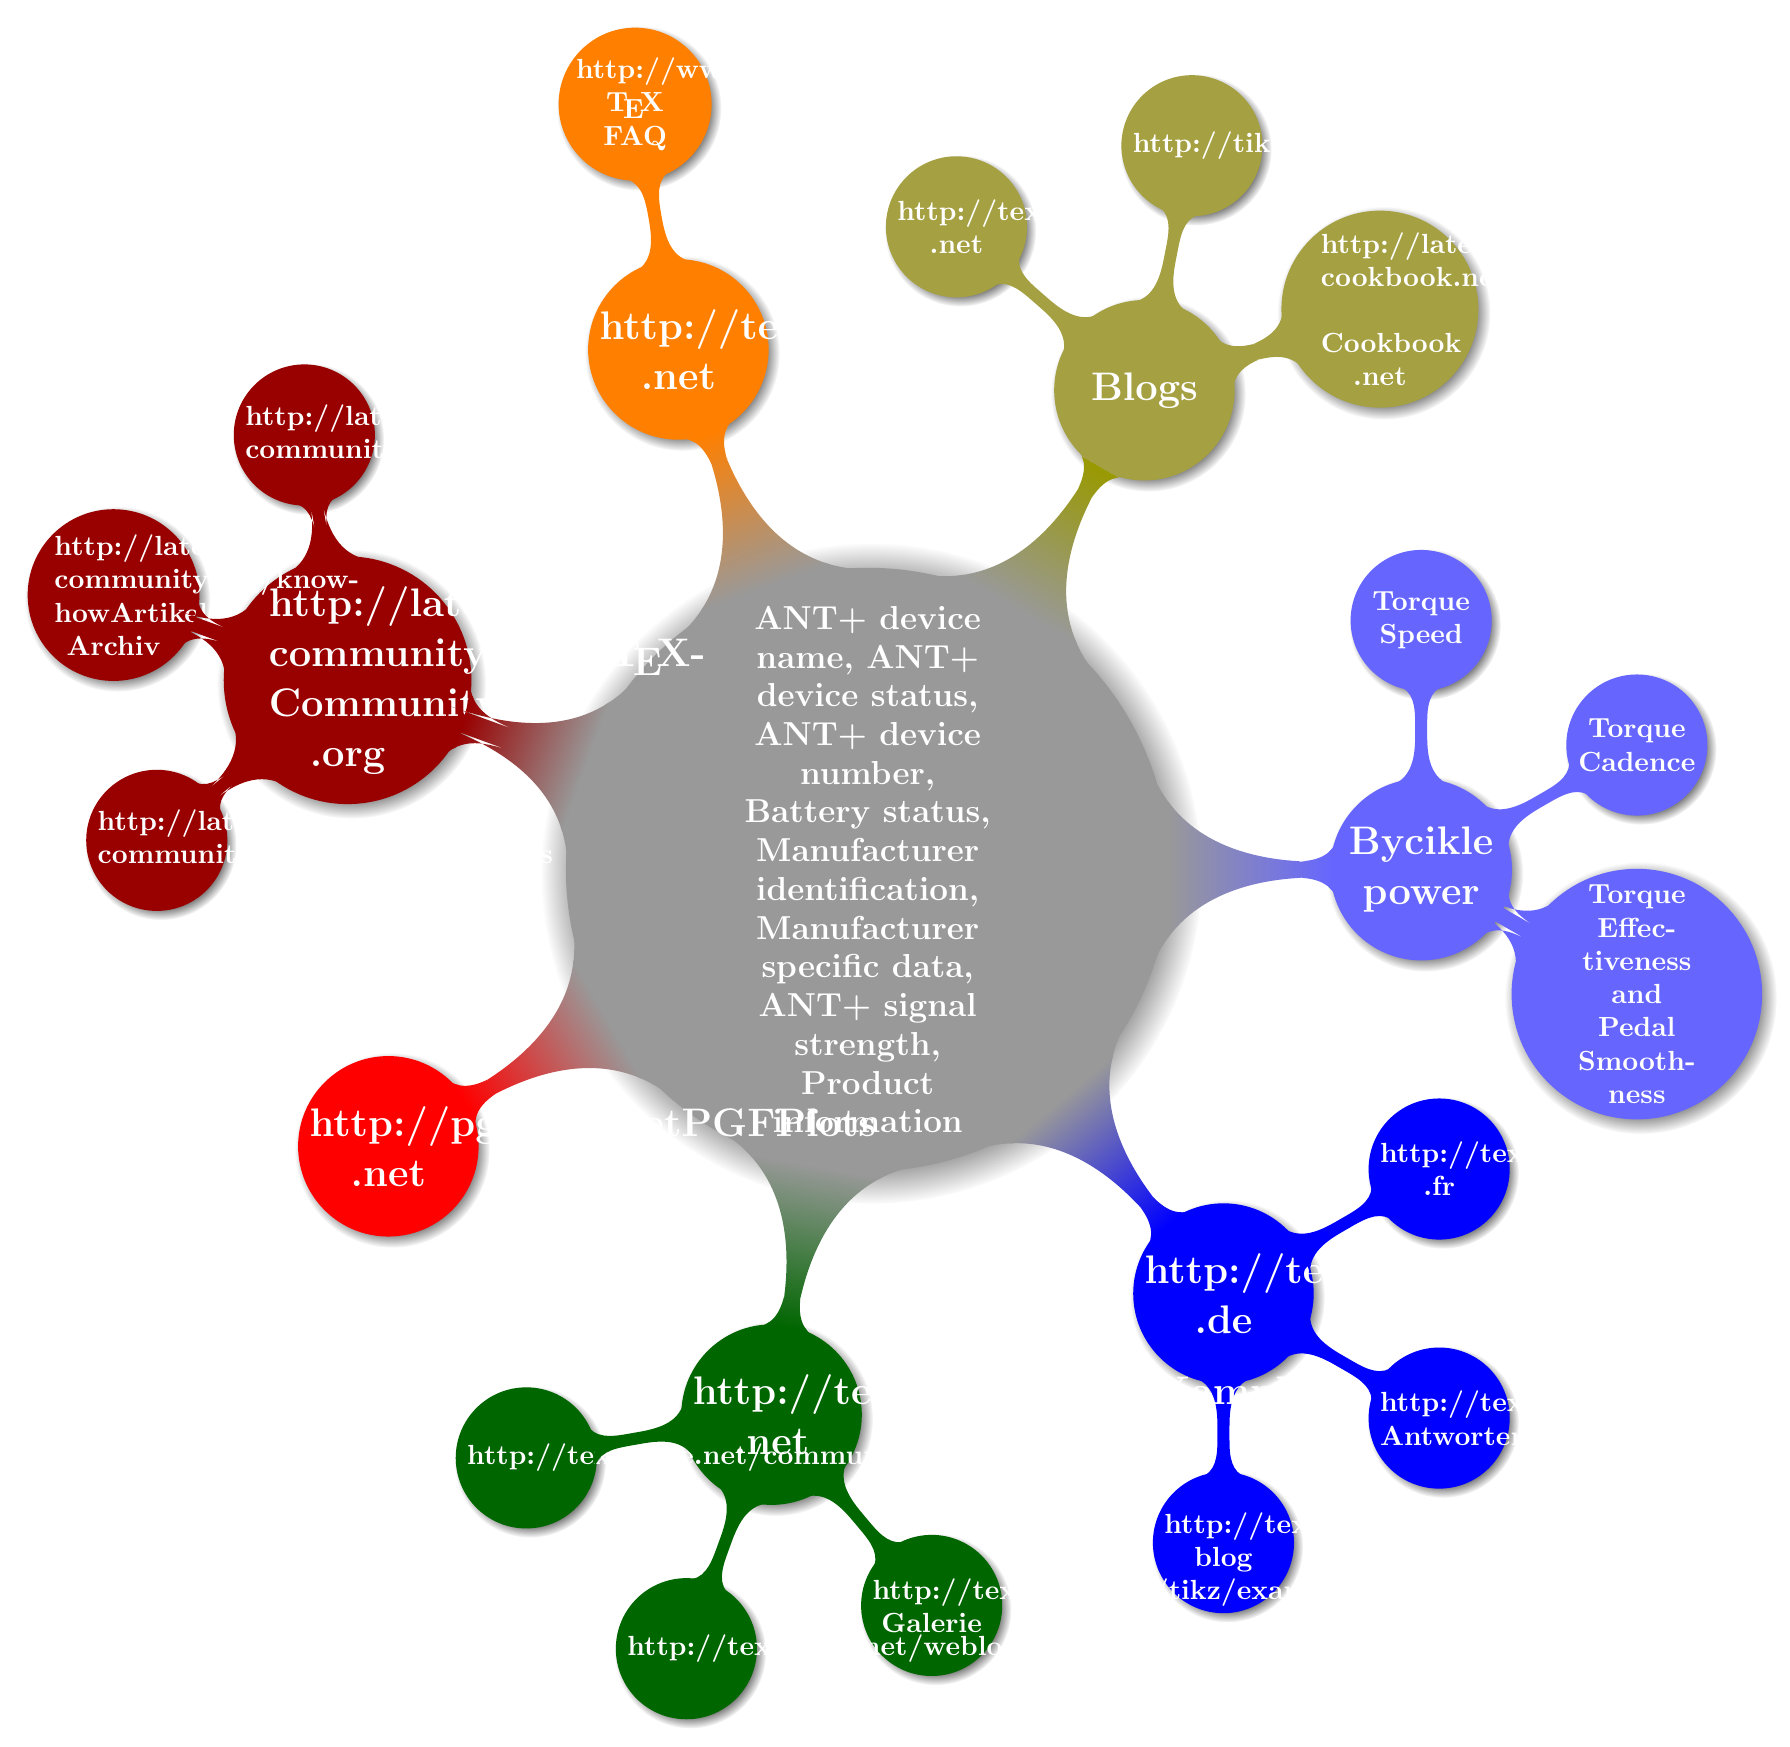
\begin{tikzpicture}[ every annotation/.style = {draw,
                     fill = white, font = \Large}]
  \path[mindmap,concept color=black!40,text=white,
    every node/.style={concept,circular drop shadow},
    root/.style    = {concept color=black!40,
      font=\large\bfseries,minimum width=10em},
    level 1 concept/.append style={font=\Large\bfseries,
      sibling angle=50,minimum width=5em,
    level distance=20em,inner sep=0pt},
    level 2 concept/.append style={font=\bfseries,level distance=9em},
  ]
  node[root] {ANT+ device name, ANT+ device status, ANT+ device number, Battery status, Manufacturer identification, Manufacturer specific data, ANT+ signal strength, Product information} [clockwise from=0]
    child[concept color=blue!60] {
      node {Bycikle power} [clockwise from=90]
        child { node {Torque Speed} }
        child { node {Torque Cadence}}
        child { node {Torque Effectiveness and Pedal Smoothness}}
    }
    child[concept color=blue] {
      node[concept] {\href{http://texwelt.de}{\TeX welt\\.de}}
        [clockwise from=30]
      child { node[concept] (TeXnique)
        {\href{http://texnique.fr}{\TeX nique\\.fr}} }
      child { node[concept] (TeXweltQA)
        {\href{http://texwelt.de/wissen/}{Fragen~\& Antworten}} }
      child { node[concept] (TeXweltBlog)
        {\href{http://texwelt.de/blog/}{User blog} }}
    }
    child[concept color=green!40!black] {
      node[concept] {\href{http://texample.net/}{\TeX ample\\.net}}
        [clockwise from=310]
      child { node[concept] (TikZGalerie) 
        {\href{http://texample.net/tikz/examples/}{TikZ-Galerie}} }
      child { node[concept] (TeXampleBlog)
        {\href{http://texample.net/weblog/}{Blog}} }
      child { node[concept] (Planet)
        {\href{http://texample.net/community/}{Planet}} }
    }
    child[concept color=red] {
      node[concept] (PGFPlots) {\href{http://pgfplots.net}{PGFPlots\\.net}}
      [clockwise from=270]
    }
    child[concept color=red!60!black] {
      node[concept] {\href{http://latex-community.org/}{\LaTeX-Community\\.org}}
        [counterclockwise from=100]
      child { node[concept] (LaTeXForum)
        {\href{http://latex-community.org/forum/}{Forum}}}
      child { node[concept] (LaTeXArtikel)
        {\href{http://latex-community.org/know-how}{Artikel-Archiv}} }
      child { node[concept] (LaTeXNews)
        {\href{http://latex-community.org/home/news}{News}} }
    }
    child[concept color=orange] {
      node[concept] (TeXdoc)
        {\href{http://texdoc.net/}{\TeX doc\\.net}}
        [clockwise from=100]
        child { node[concept] {\href{http://www.tex.ac.uk}{UK \TeX \\FAQ}}
        }}
    child[concept color=yellow!60!black] {
      node[concept] (Blogs) {Blogs} [clockwise from=139]
      child { node[concept] {\href{http://texblog.net/}{\TeX blog\\.net}}}
      child { node[concept] {\href{http://tikz.de/}{TikZ.de}} }
      child { node[concept] (Cookbook)
        {\href{http://latex-cookbook.net/}{\LaTeX-\\Cookbook\\.net}} }
    };

\end{tikzpicture}
\end{document}
